% !TEX encoding = UTF-8 Unicode
\subsection{Fase V: Validazione}
	\textbf{Periodo}: dal \insdate{10}{05}{2015} al \insdate{07}{06}{2015} \\Questa fase comincia con la fine della \insphase{Fase PROP} e termina con la scadenza della consegna per la \insrev{RA}.
	\begin{itemize}
		\item \textbf{Incremento e Verifica}: se necessario verranno effettuati aggiornamenti ai vari documenti scritti;
		\item \textbf{Validazione}: viene verificato, attraverso tracciamento, di aver soddisfatto i requisiti presenti nel documento \insdoc{Analisi dei Requisiti v1.0};
		\item \textbf{Esecuzione test}: verranno eseguiti i test di sistema previsti dal documento \insdoc{Piano di Qualifica v 7.0};
;
		\item \textbf{Correzione bug}: i bug rilevati verranno risolti;
		\item \textbf{Collaudo}: viene eseguito e completamente collaudato il sistema creato.
	\end{itemize}
	\subsubsection{Diagramma di Gantt delle attività}
		\begin{figure}[H]\centering
			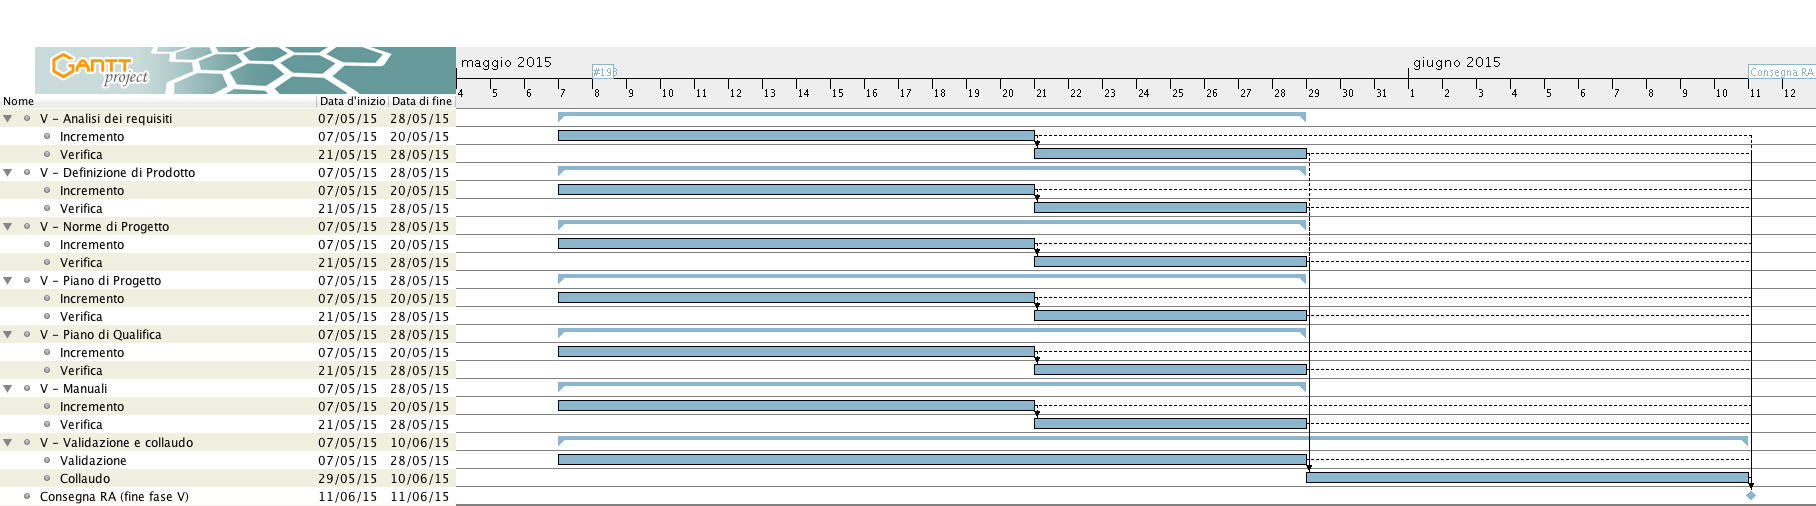
\includegraphics[width=\textwidth]{PianoDiProgetto/Pics/FaseV.png}
		\caption{Gantt Fase V}
\end{figure}
